%%%%%%%%%%%%%%%%%%%%%%%%%%%%%%%%%%%%%%%%%%%%%%%%%%%%%%%%%%%%%%%%%%%%%%%%%%%%%%%%
%%  IMPLEMENTATION
%%%%%%%%%%%%%%%%%%%%%%%%%%%%%%%%%%%%%%%%%%%%%%%%%%%%%%%%%%%%%%%%%%%%%%%%%%%%%%%%
\chapter{Implementation}\label{implementation}
This chapter focuses on the non-trivial engineering decisions and the places where a straightforward approach failed; infrastructure that works as expected is described briefly.

\begin{figure}
	\centering
	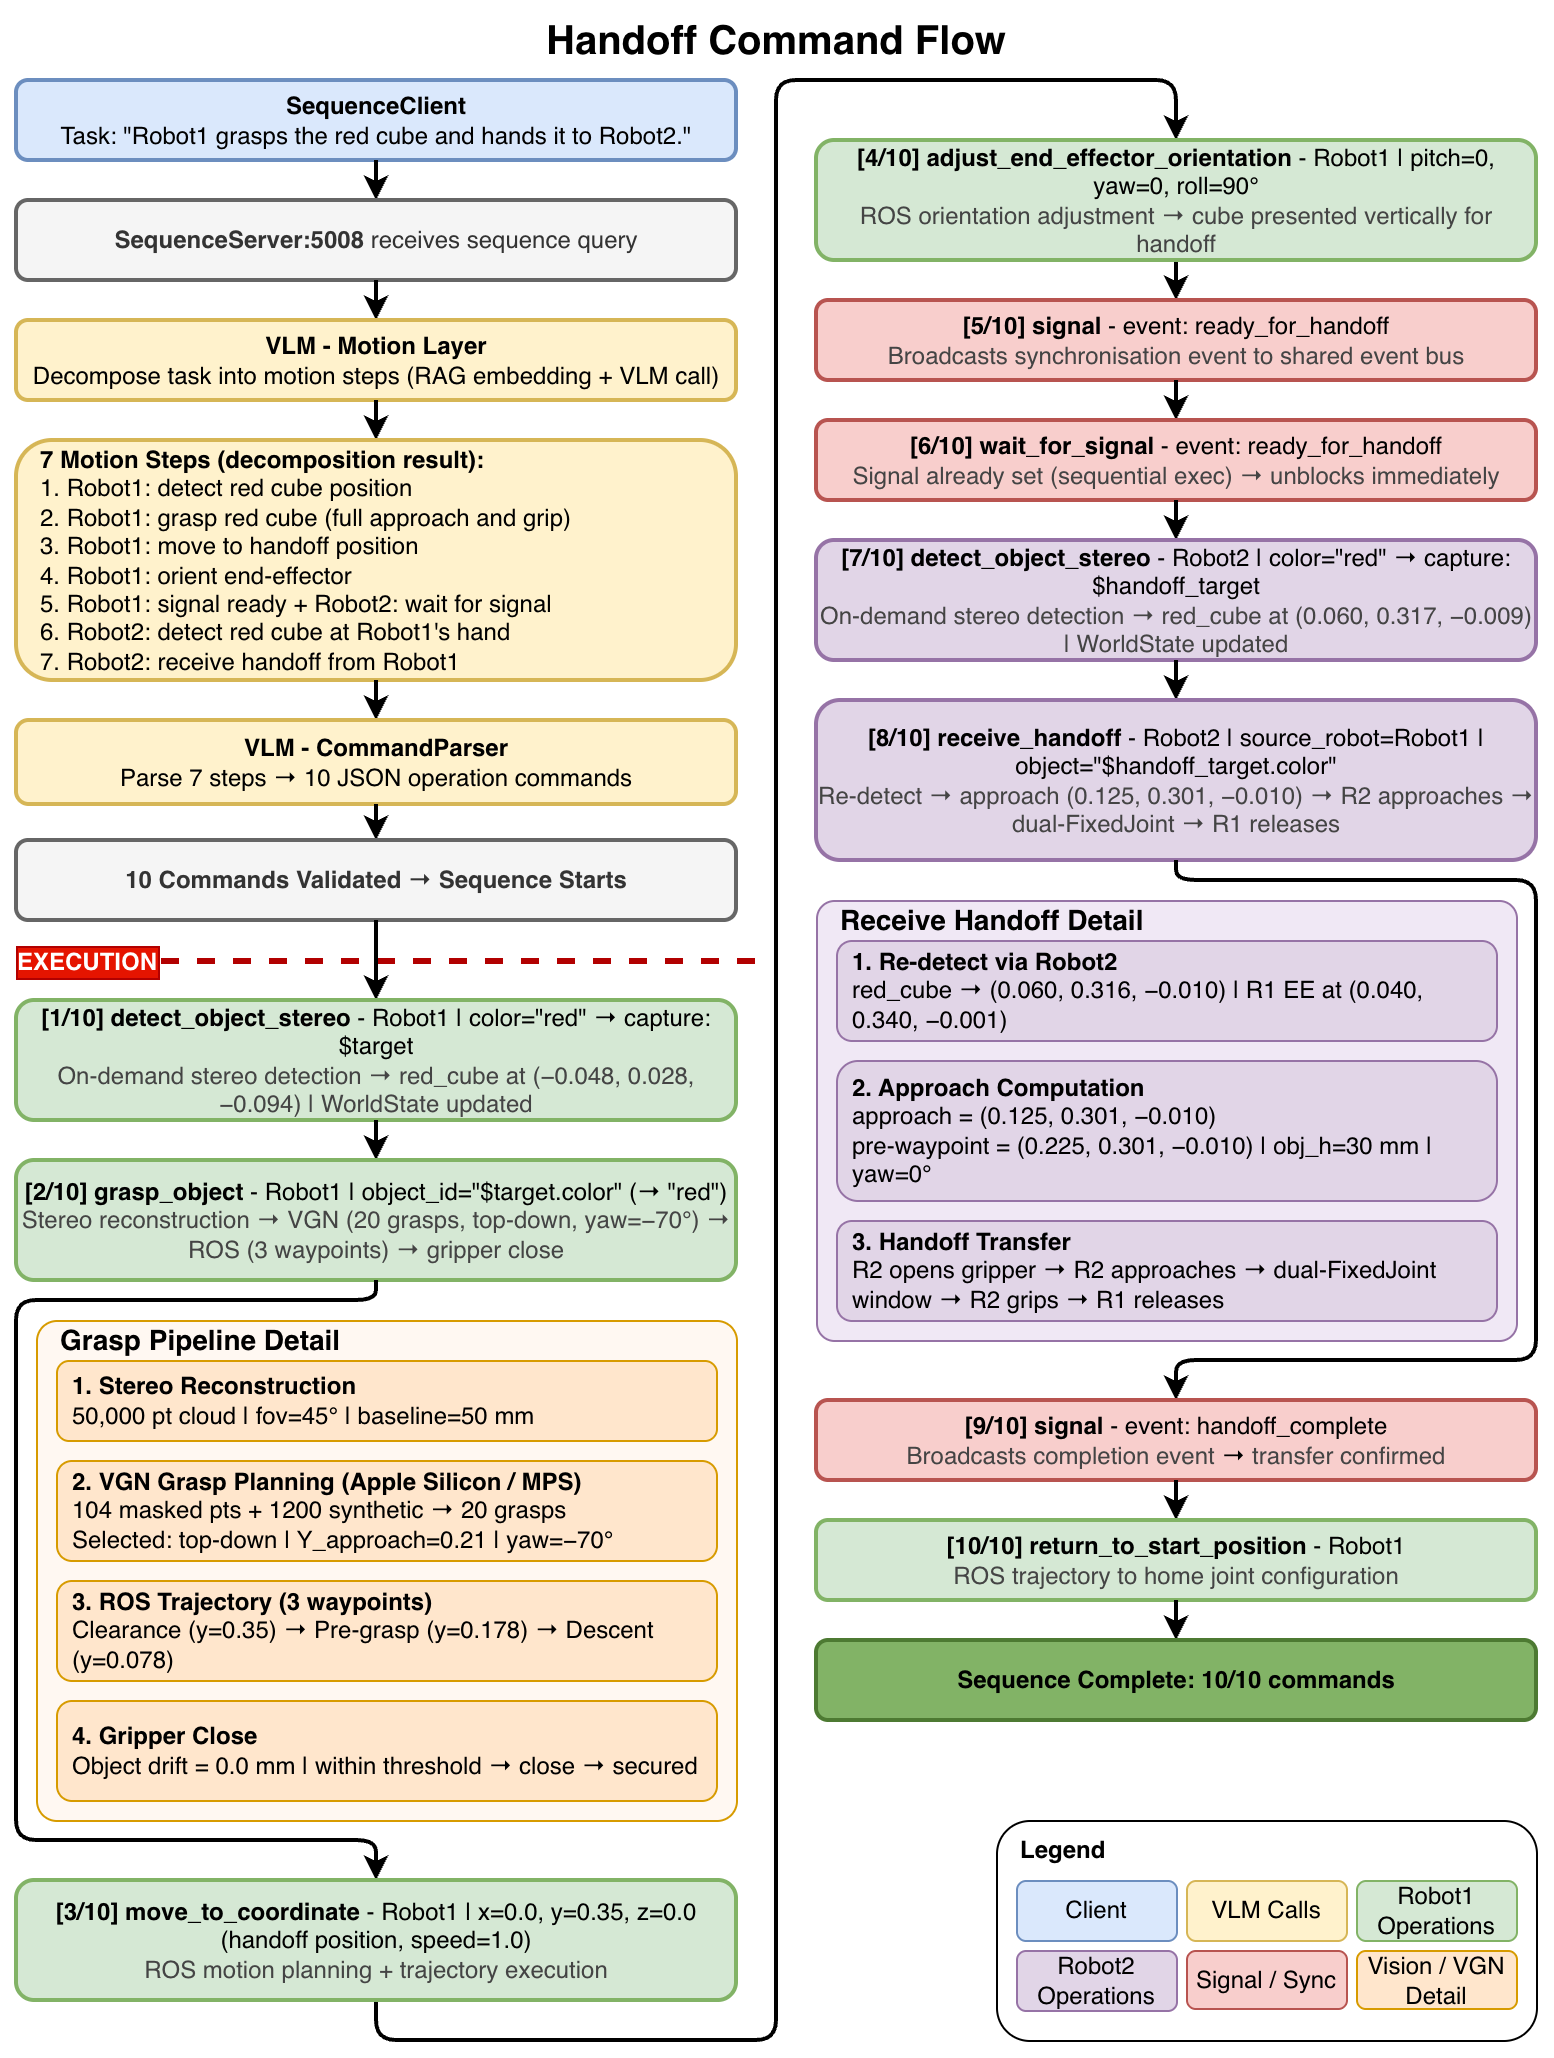
\includegraphics[width=1\linewidth]{images/12_handoff_sequence.png}
	\caption{A detailed flowgraph of how the handoff command is processed by the system.}
	\label{fig:handoff_flow}
\end{figure}

\begin{figure}
	\centering
	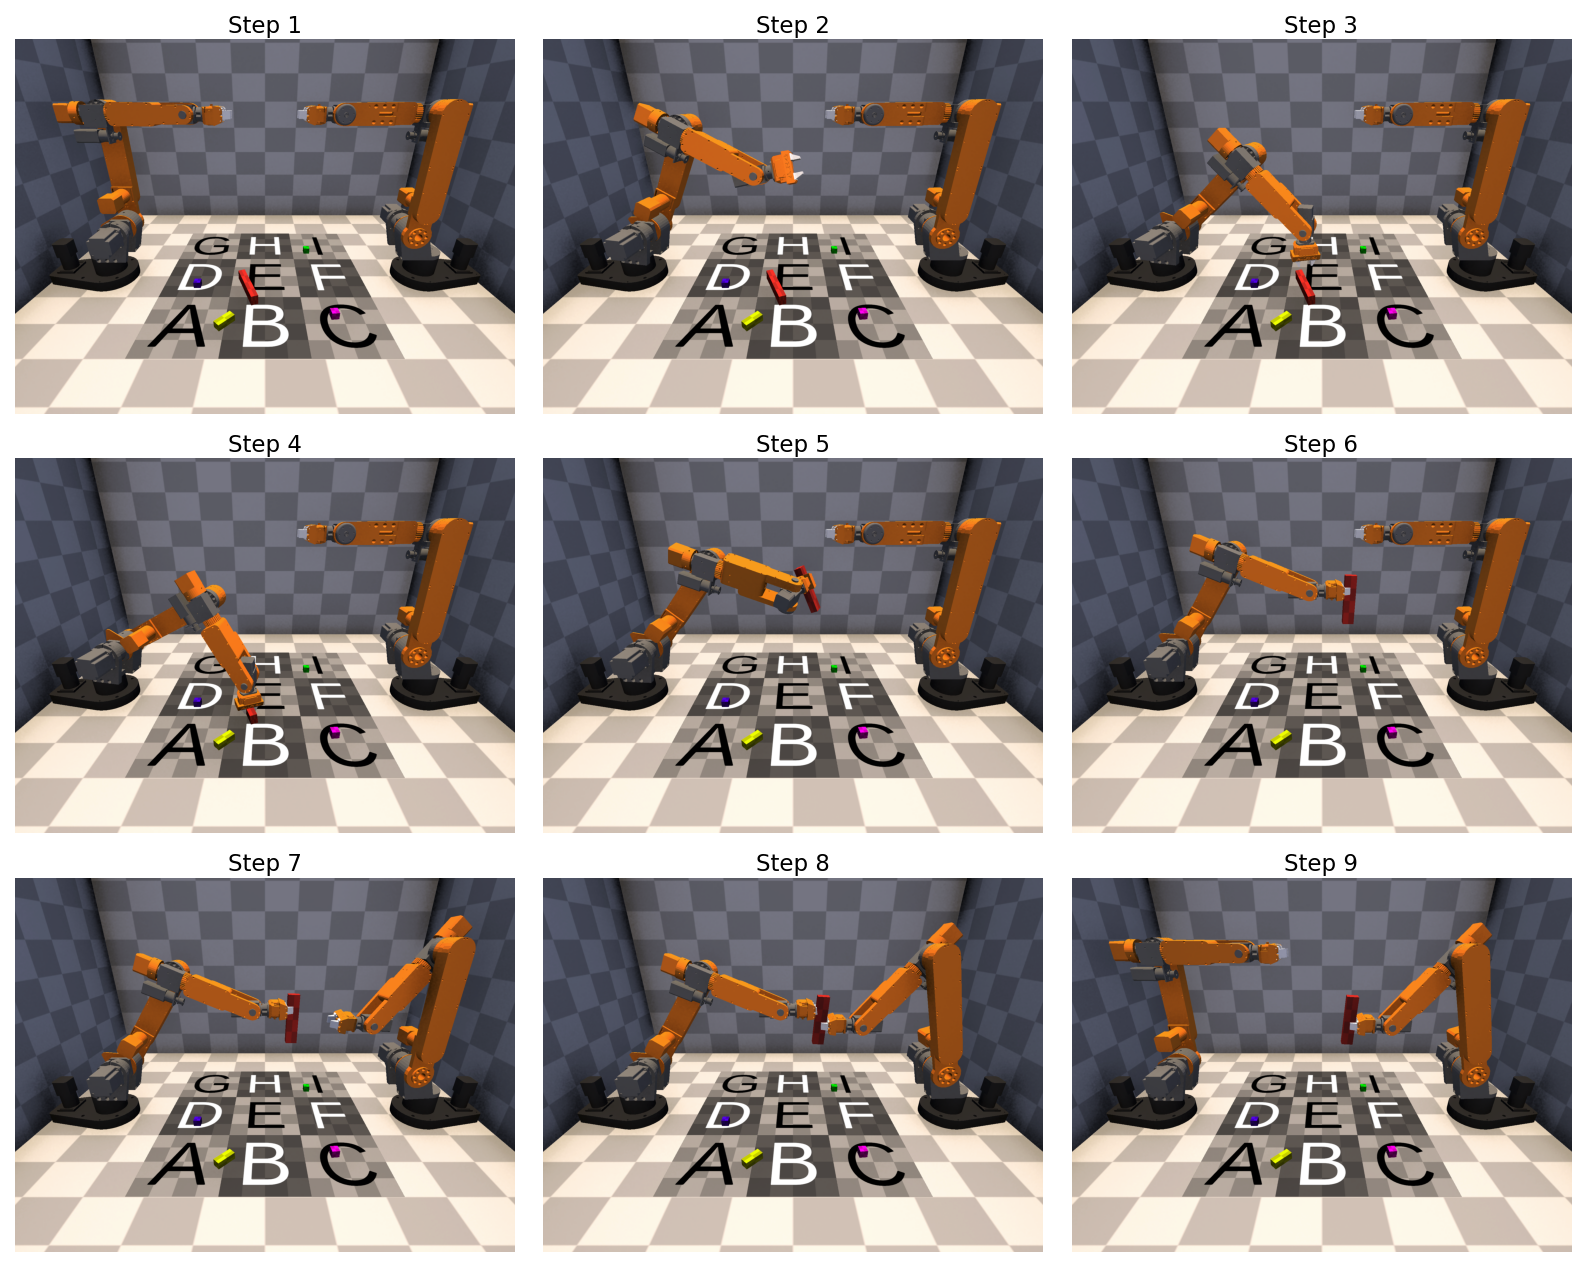
\includegraphics[width=0.75\linewidth]{images/18_handoff_sequence_example.png}
	\caption{Accompanying motion of the two robots during the handoff sequence. Note the nine steps: the \texttt{grasp\_object} and \texttt{receive\_handoff} operations each expand into internal waypoint steps.}
	\label{fig:handoff_example}
\end{figure}

Figure~\ref{fig:handoff_flow} traces a complete handoff command through most of these layers, while Figure~\ref{fig:handoff_example} shows the resulting robot motion. The flowgraph serves as a structural reference while reading this chapter, and the motion sequence illustrates the behavior the implementation produces. The full implementation is available on GitHub\footnote{\url{https://github.com/JanMStraub/Cooperative-Robot-Behavior-from-Basic-Action-Modules}}.

% ------------------------------------------------------------------------------
\section{System Infrastructure}\label{sec:infrastructure}
Before the system’s intelligent components can do anything, several foundational pieces need to be in place, especially a physics-accurate simulation environment, a motion planning backend, and a communication layer that ties Unity and Python together. The following sections describe each of these in turn, focusing on the non-obvious engineering decisions and the problems that motivated them.

\subsection{Simulation Environment and Robot Control}\label{sec:sim-env}
The simulation runs in Unity 6000.3.11f1~\cite{unity} using the \texttt{ArticulationBody} physics component to model two AR4~\cite{AnninRobotics2026} 6-DOF robotic arms (Figure~\ref{fig:robot_env}). To obtain an accurate representation of the physical robot, we imported the actual \gls{urdf} files directly into the scene. \texttt{ArticulationBody} provides reduced-coordinate dynamics, so joint behavior stays physically plausible without the numerical drift that affects traditional Rigidbody chains. Each arm is driven by a three-layer control stack, with the \gls{ik} solver at the bottom, the trajectory controller above it, and the robot controller at the top, handling convergence.

\begin{figure}
	\centering
	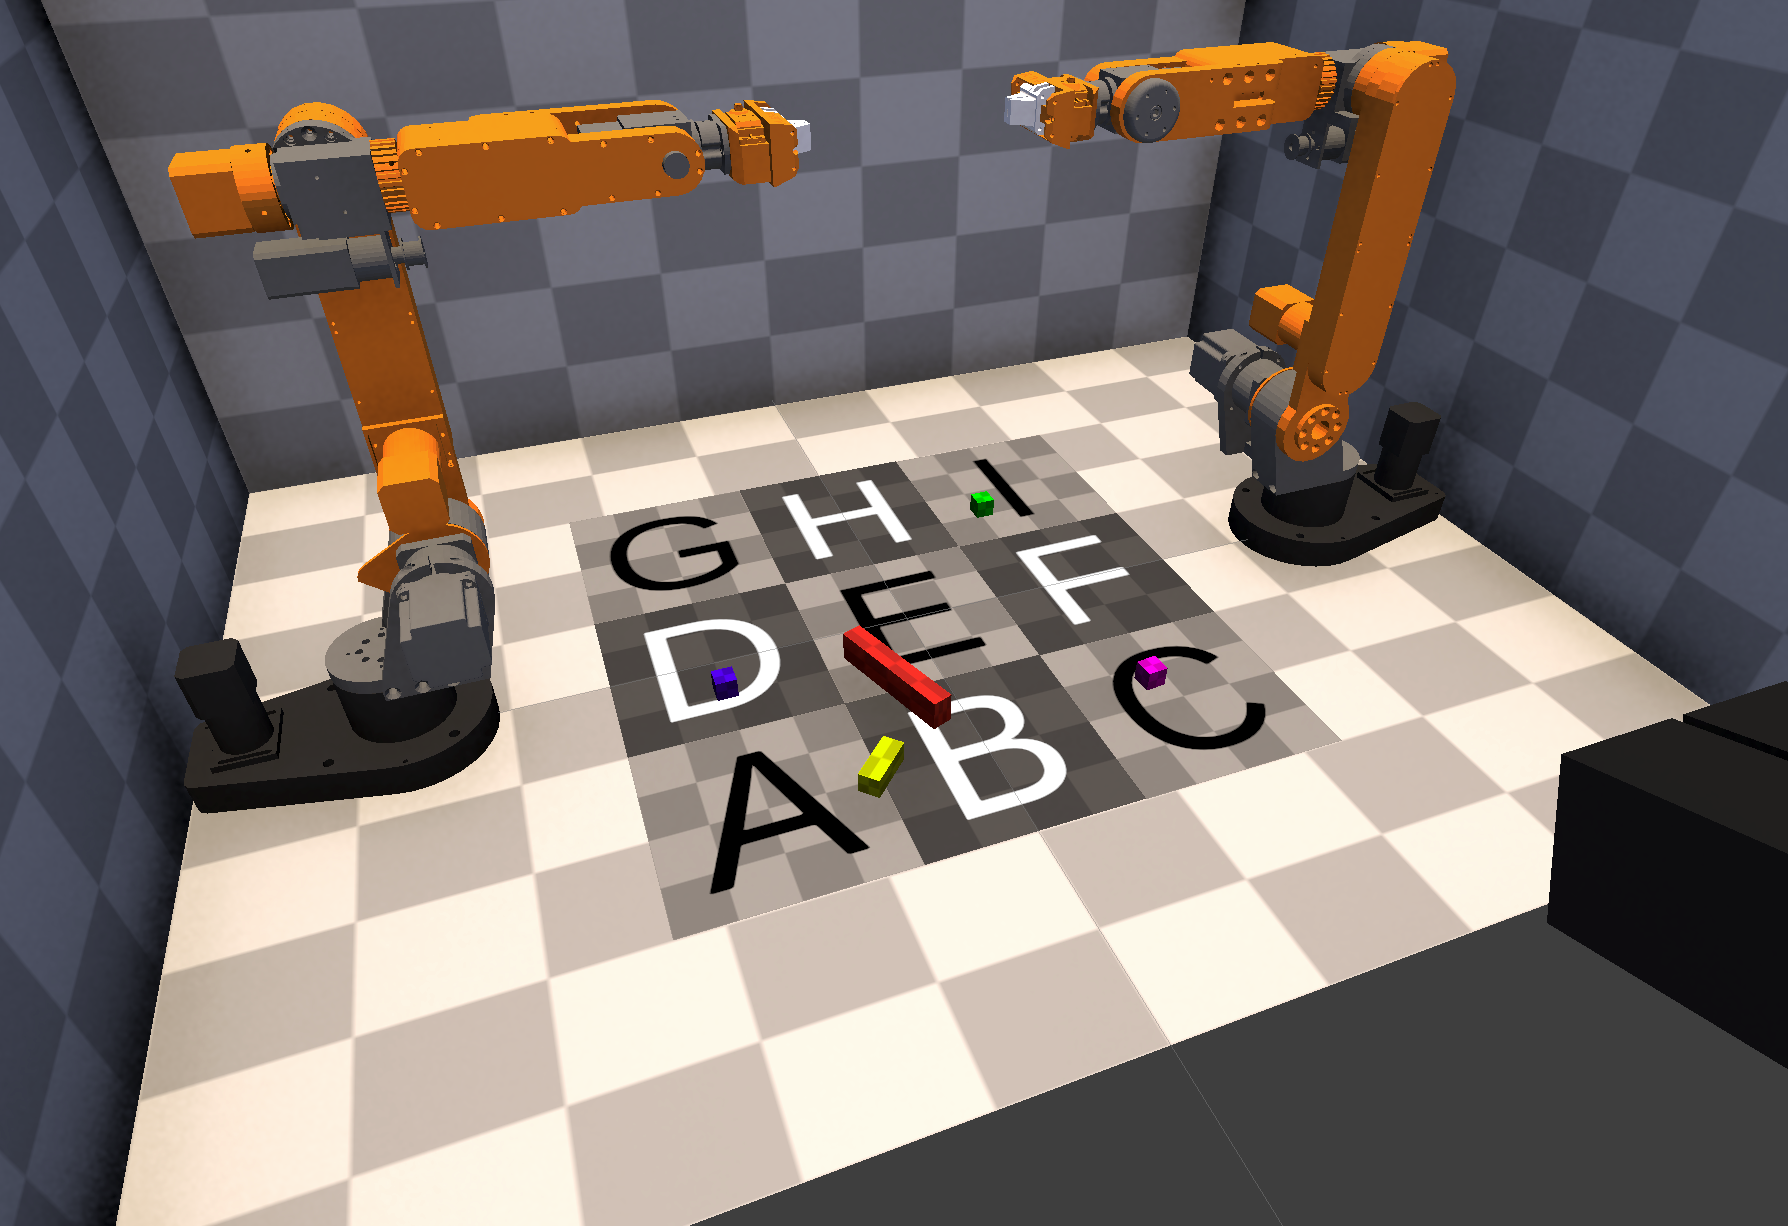
\includegraphics[width=0.5\linewidth]{images/14_robot_env.png}
	\caption{The Unity simulation environment showing the two AR4 robotic arms and the mutual workspace. Lettered zones are used to place tasks; colored objects serve as manipulation targets; and the two black boxes on the right represent the stereo camera.}
	\label{fig:robot_env}
\end{figure}

The bottom layer is the \gls{ik} solver, a damped least-squares mapping from Cartesian error to joint deltas. An earlier version oscillated due to a too-large per-frame step and insufficient damping. Adding a velocity-feedback term to the position error, turning the update into a \gls{pd} law before the damped-least-squares inverse, damped the swing. The solver maps the six-dimensional Cartesian error $e$ to a joint step $\Delta q$ through the damped pseudo-inverse
\begin{equation}\label{eq:dls}
	\Delta q = J^{\top}\bigl(J J^{\top} + \lambda^{2} I\bigr)^{-1} e,
	\qquad
	e_{\mathrm{trans}} = K_p\, e_{\mathrm{pos}} + K_d\, e_{\mathrm{vel}},
\end{equation}
where $J$ is the $6 \times n$ end-effector Jacobian, $\lambda$ the damping factor, and $I$ the identity matrix that adds $\lambda^{2}$ to the diagonal of $J J^{\top}$ to keep it invertible near singularities. The translational part of $e$ carries the \gls{pd} feedback, with $K_p$ acting on the position error $e_{\mathrm{pos}}$ and $K_d$ on its rate $e_{\mathrm{vel}}$; the rotational part is the orientation error. The translational command $K_p\, e_{\mathrm{pos}} + K_d\, e_{\mathrm{vel}}$ is clamped to unit magnitude before being combined with the orientation error and passed to the inverse, which bounds the per-step correction when a large target jump would otherwise overshoot.

We set $K_p = 3.5$ and $K_d = 0.5$. Convergence is not the solver's responsibility but the robot controller's, which declares the target reached once the position error falls below an adaptive threshold (0.02 m by default, tightened for grasping) and the orientation error is within tolerance. The remaining solver bounds are a damping factor $\lambda = 0.2$, a maximum joint step of 0.2 rad per iteration, and a joint-velocity clamp of 5.0 rad/s.

The damped least-squares solver, however, is a local, gradient-based method. It minimizes Cartesian error by following the Jacobian gradient from the current joint configuration. Because it cannot avoid local minima or reason about the global joint-space landscape, two identical Cartesian targets can produce different joint configurations and approach paths depending on the initial state, rest pose, mid-task configuration, or a previous grasp. This results in configurations near joint limits or wrist singularities that can be unreachable from some starting poses, even when they are kinematically feasible from others. Reproducibility can also suffer, as runs starting from the home pose reliably converge, while those after a sequence can land in geometrically correct but mechanically awkward configurations, increasing settling time. To fix this, multi-phase benchmarks such as B8 issue an explicit \texttt{return\_to\_start\_position} command at the end of each phase, resetting the arm to a known well-conditioned configuration before the next task.

Above the \gls{ik} solver, a trajectory controller generates trapezoidal speed curves in Cartesian space, ensuring controlled acceleration and deceleration instead of abrupt changes in target position. It operates with its own \gls{pd} gains (a position gain of 10.0 and a velocity gain of 2.0 per axis), governing how aggressively it tracks the desired profile. These gains are distinct from the \gls{ik}-level gains. The trajectory controller determines what the Cartesian target should be at any given instant, while the \gls{ik} solver translates each of those targets into joint-space commands.

We configure the \texttt{ArticulationBody} joints with per-joint stiffness and damping profiles tuned to each joint’s mechanical characteristics. Damping was tuned empirically, as the critical-damping condition $d = 2\sqrt{k \cdot I}$, where $d$ is the joint damping, $k$ the stiffness, and $I$ the rotational inertia, serves only as a lower-bound reference; at Unity’s 50~Hz physics rate, the joints require damping well above this baseline (see Appendix~\ref{appendix:robot_values}).

This three-layer control stack is only fully active in Unity mode. In the default Hybrid mode, each motion is attempted through MoveIt first and falls back to the Unity \gls{ik} and trajectory stack when planning fails, for instance, on a wrist singularity or an unreachable goal. In \gls{ros} mode, MoveIt computes every joint trajectory, Unity receives it over the \gls{ros}-TCP bridge, and the \texttt{ArticulationBody} joints execute it directly; the \gls{ik} solver and trajectory controller are bypassed entirely. The \gls{ros} implementation is described in detail in Section~\ref{sec:ros_moveit}.

\begin{figure}
	\centering
	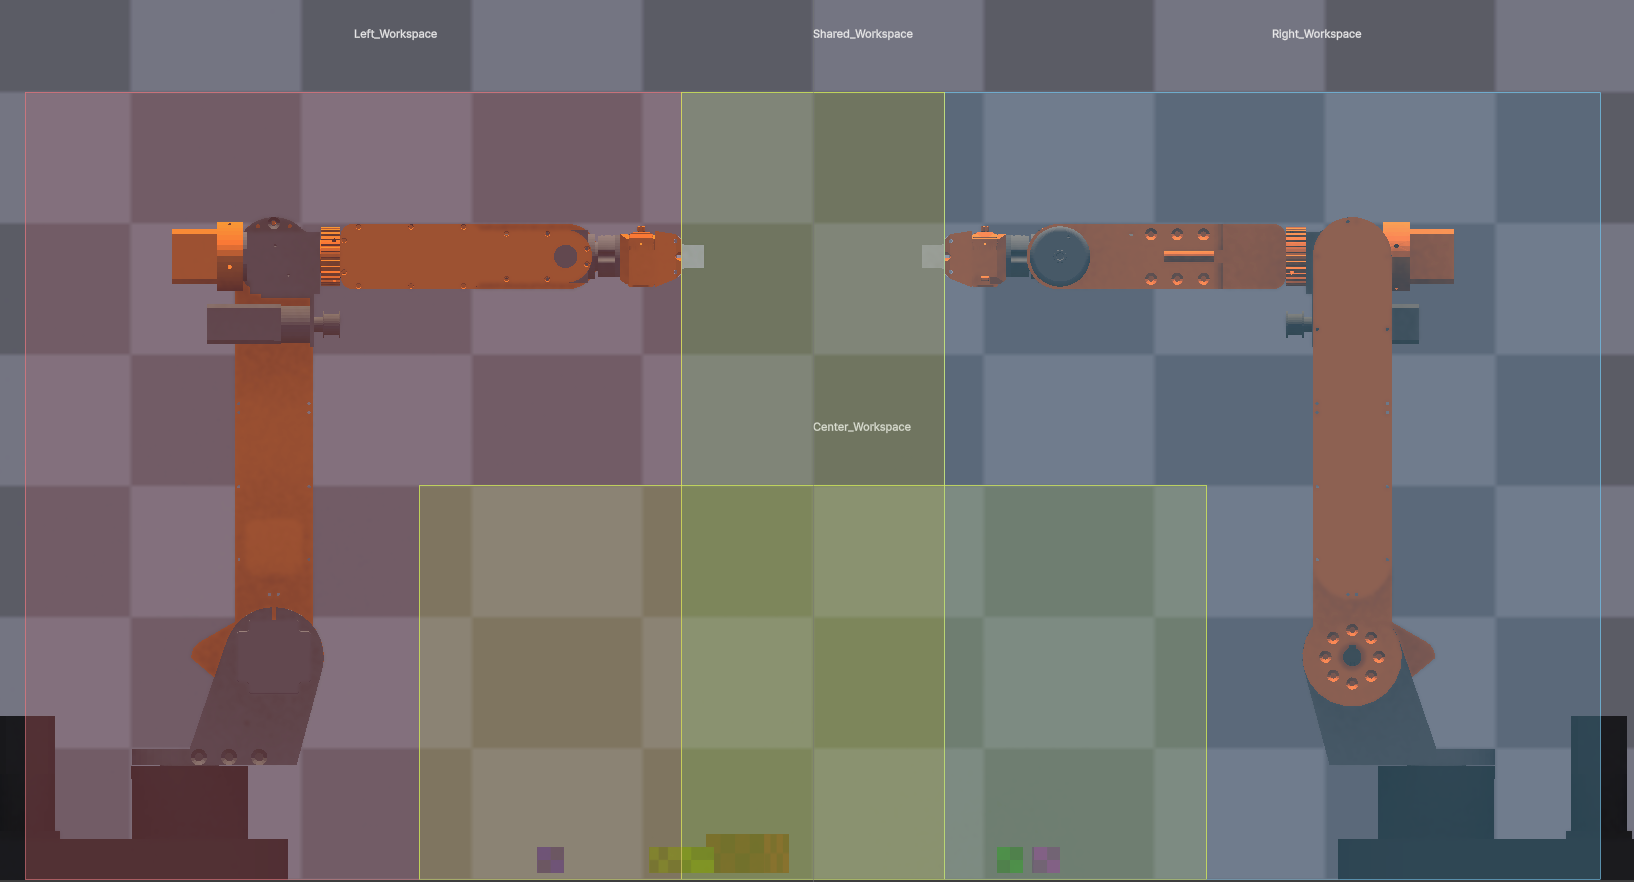
\includegraphics[width=0.75\linewidth]{images/15_robot_workspaces.png}
	\caption{Workspace regions defined in Unity, used by the \gls{kg} and the evaluation benchmarks. Red and blue mark each robot’s primary zone; the yellow areas are the center and shared zones where the two arms may interact.}
	\label{fig:robot_workspaces}
\end{figure}

Safety limitations operate in three distinct layers. At the Python level, \texttt{CoordinationVerifier} runs a static pre-check before every navigation command. If the planned target falls within 60~mm of the partner robot’s current end-effector position, the command is blocked, and a safe waypoint is prepended to the resolution suggestions before dispatch. When both robots are moving, a separate, looser check compares the two planned targets to ensure a minimum separation of 0.2~m. The same pass also checks for workspace conflicts, object conflicts (both robots targeting the same grasped object), and potential deadlocks.

At the Unity level, the \texttt{ProximityGuard} monitors end-effector separation at runtime. When their separation drops below 0.25~m, both robots freeze. Link-to-link proximity for joints 2–5 is assessed separately using a tighter 0.15~m threshold, since mid-arm collisions can occur even when end-effectors are far apart. The frozen state is broadcast to Python on the next \texttt{WorldStatePublisher} cycle, allowing the planner to replan. During intentional close-approach operations such as handoffs, the \texttt{ProximityGuard} is disabled by the \texttt{receive\_handoff} operation and re-enabled on completion, because those sequences handle inter-robot safety internally through the signal/wait serialization protocol.

The third safety layer is the workspace region system (Figure~\ref{fig:robot_workspaces}). The workspace is divided into four named regions: \texttt{left\_workspace} ($-0.6 \leq x \leq -0.1$~m, Robot~1’s main area), \texttt{right\_workspace} ($0.1 \leq x \leq 0.6$~m, Robot~2’s main area), \texttt{shared\_zone} ($-0.1 \leq x \leq 0.1$~m, the overlap of both robots’ allocations), and \texttt{center} (which overlaps the shared zone and inner parts of both workspaces and is used by the \gls{kg} for proximity reasoning). Region ownership is tracked by Python’s \texttt{WorldState}. Enforcement occurs through the \texttt{yield\_workspace} operation, which causes a robot to release its current region so the partner may enter. This strict region partition differs from the per-robot reachability bounds provided to the command-parser model in its prompt (Appendix~\ref{appendix:prompts}), which extend each arm's reachable range to $|x| \leq 0.165$~m. The difference is that the looser bound reflects the actual kinematic reach across the centerline, so the model can place and grasp objects there, while the tighter $\pm0.1$~m \texttt{shared\_zone} sets the conservative boundary at which region allocation and coordination take over.

\subsection{Grasp Planning Pipeline}\label{sec:grasp-pipeline}
Grasping is handled by a four-stage pipeline inspired by the MoveIt grasp planning architecture and implemented separately on both the Unity and Python sides. The two implementations share the same logical structure, namely candidate generation, \gls{ik} filtering, collision filtering, and scoring, but they serve different execution paths. The Unity pipeline plans for the built-in \gls{ik} stack, while the Python pipeline plans for the \gls{ros}/MoveIt path and validates its candidates directly against MoveIt’s \gls{ik} solver. Table~\ref{tab:grasp_params} lists the key parameter differences.

\begin{table}[t]
	\centering
	\begin{tabular}{lcc}
		\hline
		\textbf{Parameter}             & \textbf{Unity} & \textbf{Python} \\
		\hline
		Candidates per direction       & 10             & 8               \\
		Angle perturbation             & $\pm20^\circ$  & $\pm15^\circ$   \\
		Maximum reach                  & 0.6 m          & 0.75 m          \\
		\gls{ik} validation iterations & 250            & 50              \\
		\gls{ik} validation threshold  & 0.01 m         & 0.005 m         \\
		Depth score weight             & 0.6            & 1.0             \\
		Pipeline time budget           & 1000 ms        & 200 ms          \\
		\hline
	\end{tabular}
	\caption{Grasp planning parameters for the Unity (\texttt{GraspConfig.asset}) and Python (\texttt{grasp\_planning/GraspConfig.py}) implementations. We tuned the Unity values for PhysX execution. A generous \gls{ik} budget and a tighter 0.6~m reach keep candidates within the range where the damped least-squares solver converges reliably. The Python pipeline can afford a tighter validation threshold and shorter time budget because its candidates are checked against MoveIt’s \gls{ik} solver.}
	\label{tab:grasp_params}
\end{table}

The candidate generator produces proposals for three directions: top, front, and side. It uses approach-angle perturbations and object-size-adaptive pre-grasp distances ranging from 5 to 15 cm. Candidates pass through an \gls{ik} filter that first applies a fast distance-based reachability check and then a full \gls{ik} validation. Those that survive are evaluated by a collision filter, which samples five waypoints along the approach trajectory and performs sphere-cast checks within a 3 cm radius at each waypoint. The final scorer combines five weighted additive criteria, namely \gls{ik} quality (weight 1.0), approach direction preference (0.8), grasp depth relative to the object center (0.6 Unity / 1.0 Python), stability based on contact geometry (1.2), and antipodal quality (1.0), all scaled by an orientation-consistency multiplier. We gave the stability term the highest weight because empirical tuning showed it was the strongest predictor of whether the grasp would withstand the forces encountered during subsequent manipulation.

Grasp verification after closing is handled by a contact sensor. It tracks per-finger contact via Unity’s collision callbacks, applies a 5-frame moving average to smooth physics noise, and requires a minimum contact duration of 50~ms and an estimated contact force above 5~N before declaring a successful grasp.

The \gls{vgn} pipeline~\cite{breyer2021volumetricgraspingnetworkrealtime} is an optional learned backend for 6-DOF grasp-pose prediction, retained as sim-to-real infrastructure and not the currently active alternative to the heuristic planner. It takes a \gls{yolo} bounding box, constructs a masked point cloud, builds a \gls{tsdf} volume, and runs \gls{vgn} inference to produce 6-DOF grasp poses, which are injected into the same filter and scorer pipeline. The executed orientation, however, is a top-down override described below, while the grasp position is taken from the detected object center. In this simulation, the center is supplied by the \texttt{WorldState} oracle rather than recovered from the point cloud, since the per-pixel depth needed to localize it from stereo is unreliable on Unity's textureless surfaces (Section~\ref{sec:perception-depth}). The measurable benefit of enabling the \gls{vgn} path therefore comes from this positioning, not from \gls{vgn}'s predicted pose (Section~\ref{sec:results-vgn}).

We first tried Contact-GraspNet~\cite{sundermeyer2021contactgraspnetefficient6dofgrasp} as the data-driven backend. However, it requires a dedicated GPU for inference, which we did not have in our development environment, so we adopted \gls{vgn} instead. Its lighter inference footprint runs on the CPU and Apple Silicon without modification, aligning with the infrastructure-independent deployment goals in Section~\ref{sec:local}. Although \gls{vgn} is trained on both top-down and side grasps, the sparse \gls{tsdf} volumes produced by this system’s stereo disparity rarely yield a confident near-vertical prediction. Our pipeline, therefore, imposes a top-down orientation unless \gls{vgn}'s predicted approach is strongly vertical ($|Y| \geq 0.7$); otherwise, the predicted approach is discarded and replaced with a straight-down grasp whose yaw is derived geometrically from the object’s long axis. Under this system’s stereo depth, the threshold is seldom met, so most executed grasps are top-down by override, not \gls{vgn}'s own preference.

\subsection{Robot Operating System and MoveIt Integration}\label{sec:ros_moveit}
The key implementation choice is to enable the \texttt{plan\_only} flag in the MoveGroup goal. MoveIt produces a joint trajectory plan but does not attempt to execute it, and Unity receives it over the \gls{ros}-TCP bridge and runs it through its \texttt{ArticulationBody} physics. The rationale for this planning-only split is given in Section~\ref{sec:ros}.

The three control modes introduced in Section~\ref{sec:sim-env} vary mainly in planning cost and collision handling. \gls{ros} mode plans through MoveIt, with trajectory execution averaging about 5~s per motion (Table~\ref{tab:b16-results}), and it provides full collision-aware planning via \gls{ompl}~\cite{6377468}. Unity mode is preferable when lower latency is required, and collision-aware planning is not needed, while \gls{ros} mode becomes worthwhile once the workspace is cluttered enough to need collision-free planning; Hybrid, the default, blends the two.

Joint states are published at 50~Hz using pre-allocated \gls{ros} messages to avoid garbage-collection pressure. Trajectories are received and validated against joint limits and velocity constraints. They are then interpolated to Unity’s fixed-update frequency. In dual-robot mode, all topics are namespaced per robot to keep the two control streams independent.

We encountered three failure modes during integration. Each required an explicit fix before the \gls{ros}/MoveIt path became reliable.

\paragraph{MoveIt \texttt{UNKNOWN\_ERROR\_99999}.}
\gls{ompl} aborted planning with error code 99999 in two distinct scenarios. First, Unity’s \texttt{ArticulationBody} physics can overshoot joint limits at the end of a trajectory, particularly after a settle timeout. Because those out-of-bounds values were submitted as the MoveIt start state, \gls{ompl} rejected it as kinematically invalid; our fix clamps every joint value to its \gls{urdf} bounds before constructing the \texttt{RobotState} message. Second, setting \texttt{is\_diff = false} at the start state caused unlisted joints to default to zero, placing the robot in self-collision or in contact with the ground plane and triggering the same error. Setting \texttt{is\_diff = true} instructs MoveIt to apply the provided joints as a differential update over its internally tracked state, leaving unlisted joints unchanged. Additionally, gripper jaw joints published by Unity must be stripped from the start state prior to submission, because the \texttt{arm} planning group does not include them, and their presence renders the start state invalid.

\paragraph{Execution settle timeout.}
Unity sends a \texttt{completed\_with\_timeout} status when trajectory execution finishes, but the arm has not fully settled at its drive target within the allotted window. If the next plan is requested immediately, MoveIt receives a stale \texttt{/joint\_states} that still reflects the arm mid-motion, resulting in a start state that either violates joint bounds or is in an unexpected configuration. Our fix inserts a 3~s physics-settle wait after any \texttt{completed\_with\_timeout} response before the next planning request is issued. The execution timeout itself is set dynamically as
\begin{equation}
	t_{\mathrm{exec}} = \max\bigl(c_0,\; 2.5 \cdot t_{\mathrm{traj}} + c_1\bigr)~\text{s},
\end{equation}
where the floor $c_0$ and offset $c_1$ are set per call path (for example, $c_0 = 30$, $c_1 = 15$ on the primary plan-and-execute path), so the timeout scales conservatively with trajectory duration.

\paragraph{\gls{vgn} approach bias.}
When stereo point cloud quality is insufficient to produce reliable \gls{tsdf} input, \gls{vgn}'s predicted approach vectors bias toward the horizontal; selecting the highest-scoring candidate unfiltered then rotates the wrist into a twisted configuration that the planner rejects. The fix is the $|Y| \geq 0.7$ vertical-component threshold described above. Near-vertical predictions are trusted; all others are overridden with the top-down direction.

\subsection{Communication Architecture}\label{sec:communication}
The Unity simulation and the Python backend communicate over TCP. All messages use a protocol that prepends a 5-byte header to each message: one byte for the message type and four bytes for the request identifier. The request ID enables asynchronous request-response matching. The Python backend maintains per-request queues and handles concurrent operations from multiple robots without mixing replies.

World state is published on a dedicated port as a one-way broadcast stream with a fixed request ID of zero, explicitly separating it from the request–response channel. We introduced this separation after early versions suffered correlation errors. High-frequency world-state updates arrived interleaved with command responses.

End-to-end, a command flows as follows. A natural-language sequence arrives at the Python \texttt{SequenceServer}; the backend passes it to the command parser; the parsed plan is sent to the sequence executor, which dispatches each operation via the \gls{ros}-Unity router. In the default Hybrid mode, motion commands are planned by MoveIt and the resulting trajectory is executed by Unity through its \texttt{ArticulationBody} physics. If planning fails, the system falls back to the Unity \gls{ik} pipeline. Unity then returns a completion notification. In practice, model parsing is the dominant fixed cost. The median time from query arrival to a validated plan was roughly 20~s, limited by the reasoning model’s thinking budget. Motion planning adds well under 0.5~s on the \gls{ros} path, or 5–10~ms per \gls{ik} step on the Unity path. Robot movement adds 2–10~s per motion command, depending on travel distance, so a single-robot command sequence typically finishes within 30–60~s of arriving, while dual-robot handoff sequences extend to roughly 60–100~s.

On top of this TCP backbone sits an optional operator interface, the Mission Control dashboard. It acts purely as a client of the existing backend. It renders the live scene from the world-state broadcast, streams logs and AutoRT task proposals, accepts natural-language commands, and exposes the benchmark analysis tab used in Chapter~\ref{evaluation}.

% ------------------------------------------------------------------------------
\section{Operations System}\label{sec:ops-impl}
Each operation is an instance of the \texttt{BasicOperation} dataclass, configured with an implementation callable; its shared \texttt{execute()} method validates parameters and dispatches to that callable, returning an \texttt{OperationResult} containing a success flag, an optional error dictionary, and a result dictionary. Operations are registered in a central registry at startup, which serves as the single source of truth for the \gls{rag} indexer, the command parser prompt, and the AutoRT task generator.

Beyond the operation implementations themselves, each operation carries structured metadata that the \gls{rag} system actively uses. \texttt{ParameterFlow} objects declare how output fields of one operation map onto input parameters of another, allowing the retrieval step to surface both the most relevant individual operation and the natural sequences it belongs to. Seven such flows are defined across the registry, covering vision, field, and spatial operations. In addition, \texttt{OperationRelationship} objects declare which operations are commonly paired together and what temporal ordering constraints exist between them.

An example of an operation can be found in Appendix~\ref{appendix:operation_example}.

% ------------------------------------------------------------------------------
\section{Intelligent Task Planning}\label{sec:planning-impl}
This section covers the concrete implementation of the command pipeline described in Section~\ref{sec:command-pipeline}, covering how we serve and configure the local model, build and query the \gls{rag} index, and convert a retrieved plan into robot actions.

\subsection{Local Model Selection}
The locally hosted \gls{vlm} is served via LM Studio~\cite{lmstudio}, which exposes an OpenAI-compatible API endpoint. We chose this interface because it lets the same client code target different models without modification, making model substitution straightforward during evaluation. Temperature is set to 0.3 for command parsing, low enough to keep plan generation predictable. For multi-step tasks, we use two complementary mechanisms to improve output quality. The first is a model-level thinking block, enabled via LM Studio’s \texttt{budget\_tokens} parameter, that lets the model reason internally before producing a response; the second is a chain-of-thought context injected into the prompt as motion-planning guidance. Together, these reduce structural errors in the generated plans, though we have not independently measured the effect of each mechanism.

\subsection{Retrieval-Augmented Generation System and Embedding}
Embeddings are generated using \texttt{nomic-embed-text-v1.5}~\cite{nussbaum2025nomicembedtrainingreproducible}, served locally via LM Studio and producing 768-dimensional vectors. The vector store uses cosine similarity search with an in-memory index protected by a thread-safe lock; the index is persisted to disk, so re-indexing is needed only when operations change. Query results are filtered using a minimum similarity threshold of 0.5 and a configurable confidence strategy (strict/balanced/permissive). If LM Studio is unavailable at startup, the system falls back to \gls{tfidf} with a maximum of 500 features, which is coarser, but sufficient to keep the system functional in degraded conditions. Figure~\ref{fig:rag} shows the indexing and search pipeline.

\begin{figure}
	\centering
	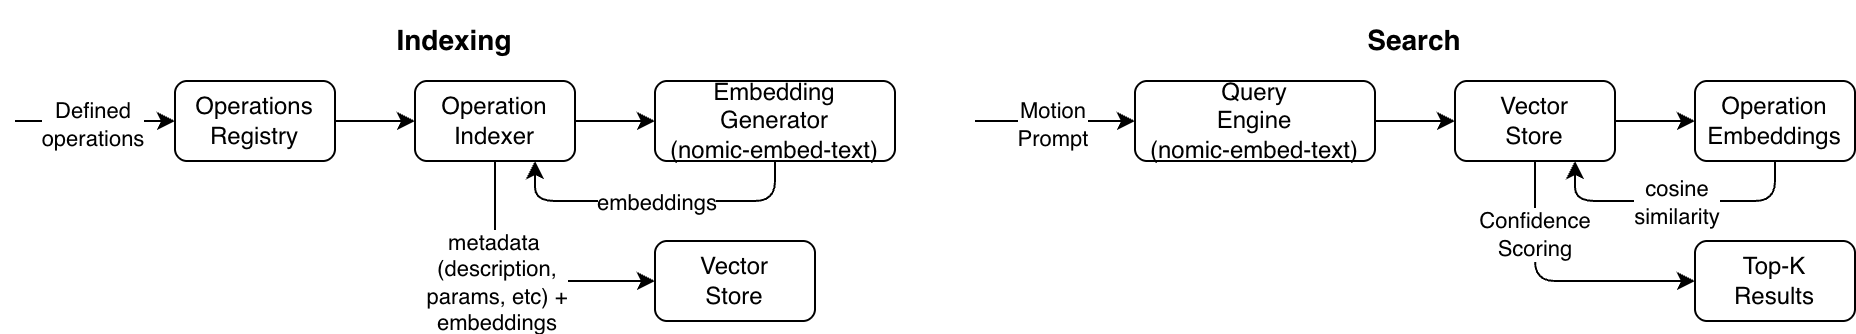
\includegraphics[width=1\linewidth]{images/13_rag.png}
	\caption{Indexing and search in the \gls{rag} system: operations are embedded and stored at startup (left); a user prompt is embedded and matched by cosine similarity, then confidence-scored to Top-K results (right).}
	\label{fig:rag}
\end{figure}

The \gls{rag} index contains 31 items in total: the 20 registered operations, 7 predefined workflow patterns, and 4 multi-robot context documents. The workflow patterns describe common multi-step sequences in a structured format, including pattern-level success criteria and failure recovery hints. When one pattern scores highly during retrieval, it is injected into the model prompt as an example plan, reducing structural errors in generated plans for familiar task types. The context documents cover workspace layout, coordination patterns, safety restrictions, and parallel execution guidelines, providing the model with relevant background when no single operation is a close semantic match for the query.

\subsection{Command Parser and Sequence Executor}
The command parser extracts and normalizes the JSON from the model’s response. Per request, a 90-second timeout is applied, and a connection pool with 10 persistent connections reduces TCP overhead. The system prompt lists the top \gls{rag}-retrieved operations with their full parameter schemas. The vector store is queried for 10 candidates spanning both operations and workflow patterns. These candidates are partitioned by type; up to 5 operations and up to 3 workflow patterns are retained, and any surplus is discarded. The most relevant items, together with critical rules for multi-robot tasks and the variable-passing syntax, are then fed into the prompt.

Before execution, the parser validates the returned plan. Operation names are checked against the registry, and every \texttt{wait\_for\_signal} call must have a matching \texttt{signal} with the same identifier. Variable references are resolved at execution time; unresolved references fall back to recovery patterns or are left for the operation’s parameter type-check to reject, and missing \texttt{capture\_var} declarations are inferred from downstream \texttt{\$var} usage. If the response can be partially salvaged, for example, if the model returned a bare array instead of a wrapped object, a normalization step is attempted before returning an error. If LM Studio~\cite{lmstudio} is entirely unreachable, the parser falls back to a regex-based matcher that covers a subset of common command patterns.

The sequence executor iterates over the validated plan. For operations sharing the same parallel group identifier, it dispatches them concurrently and blocks until all complete or a timeout elapses. Variable passing is handled automatically. After each operation, result fields declared in the operation’s parameter flow metadata are stored in a session-scoped variable dictionary; before each operation, missing parameters are filled from this dictionary by field-name matching. Both explicit capture directives in the plan and automatic capture run in sequence, with explicit directives applied first. Signal and wait primitives are implemented using a \texttt{threading.Condition} variable. The signaling robot calls \texttt{notify\_all()} on the condition, and the waiting robot blocks on the condition until notified.

\subsection{Reflection Strategy}\label{sec:reflection-impl}
When an operation fails, the executor checks whether it qualifies for reflection-based recovery. Only Navigation, Manipulation, and Perception operations are eligible; synchronization primitives and status checks are explicitly excluded, since re-querying the language model for them offers no benefit and adds latency. If the failed operation is eligible and reflection is enabled, the executor constructs a failure hint by combining the error message with any recovery suggestions returned by the failed operation. This hint is returned to the command parser alongside the original natural-language command, which re-queries the \gls{vlm} with the failure context appended. The re-parsed command is re-resolved against the current variable store and re-executed. By default, this loop runs up to 2 retries; on success, the failed entry in the sequence log is replaced with the successful result, and execution continues normally.

\subsection{Knowledge Graph}\label{sec:kg-impl}
The \gls{kg} is implemented as a thread-safe directed multi-graph that permits safe access from the world-state callback thread and from operation handlers. The graph is updated in place on every world-state update by a builder that registers as a callback on the world-state server. Three node types represent robots, objects, and workspace regions. Six edge relations are actively populated: \textsc{Can\_Reach}, \textsc{Near}, \textsc{In\_Region}, \textsc{Grasping}, \textsc{Adjacent\_To}, and \textsc{Allocated}. Figure~\ref{fig:kg_example} shows the graph state at simulation start.

\begin{figure}
	\centering
	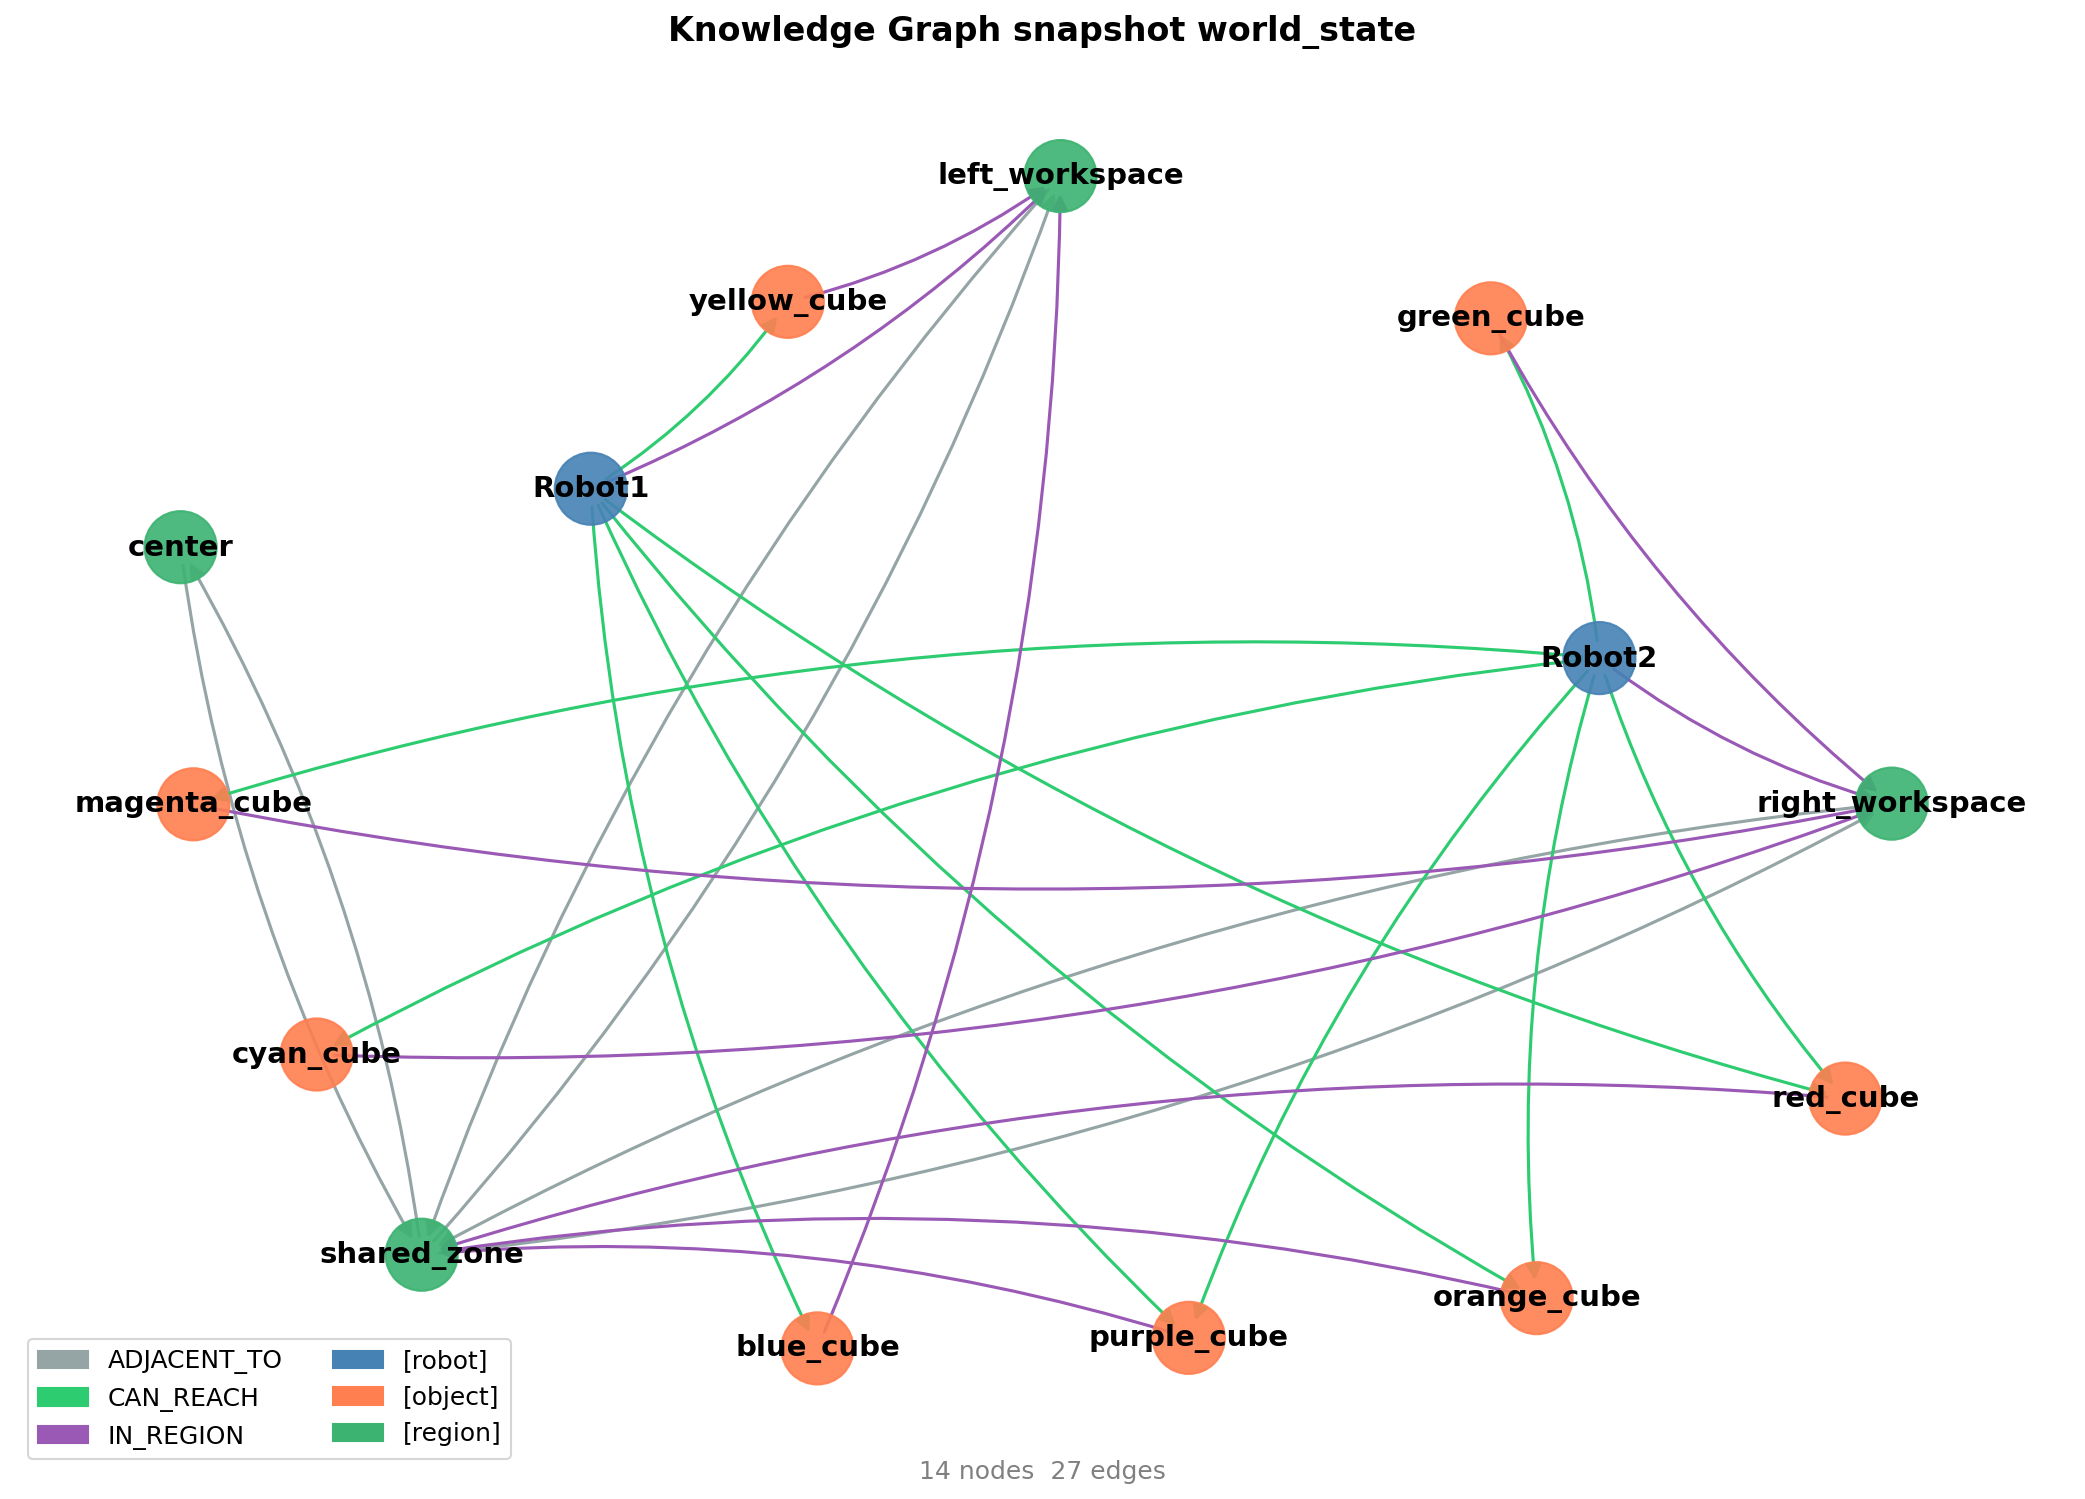
\includegraphics[width=0.75\linewidth]{images/11_kg_world_state.png}
	\caption{The \gls{kg} at simulation start: robot, object, and region nodes with their initial reachability, proximity, and containment edges.}
	\label{fig:kg_example}
\end{figure}

% ------------------------------------------------------------------------------
\section{Benchmark Implementation}\label{sec:benchmark-impl}
Each benchmark is implemented as a self-contained Python module. The single-task benchmarks (B1–B7, B9, B10) expose a \texttt{get\_task()} function that returns one natural-language task; the ablations (B11–B16) expose \texttt{get\_tasks()} returning a list, and B8 exposes \texttt{get\_sub\_tasks()}. The \texttt{BenchmarkRunner} dispatches this string to the live system over the same TCP interface used in normal operation, connecting to the \texttt{SequenceServer}. Most execution benchmarks send the task string through the full parsing pipeline. Two exceptions, B15 (\gls{vgn}) and B16 (\gls{ros}-vs-Unity), dispatch fixed operation chains directly to the sequence executor and bypass the command parser so that grasp quality and movement timing are measured independently of parser variability. For the rest, the command parser translates the natural-language instruction into an ordered list of operations, which the sequence executor then executes in the simulation.

Three benchmarks stop earlier in the pipeline. B9 runs in parse-only mode to evaluate input rejection, and the B11 and B14 ablations evaluate parse quality without dispatching operations to Unity. B17 is the most self-contained of all. It bypasses the \texttt{BenchmarkRunner} dispatch entirely and drives \texttt{RobotConstitution.evaluate\_task()} and the task generator in process, so it runs fully offline with only the local model and no Unity or server stack (Section~\ref{sec:results-autort}).

Results are collected as a \texttt{BenchmarkResult} dataclass that captures step-level metrics, operation name, duration, success flag, and error information, along with aggregate figures: total wall-clock duration, operations executed and succeeded, per-benchmark success rate, mean step duration, and the index of the first failing step. Each run is tagged with a unique identifier that combines a UTC timestamp and a fragment of a universally unique identifier (UUID), enabling each run to be traced. A run is marked successful if and only if the sequence executor reports success for the entire sequence, inheriting the operation-level pass/fail semantics already defined in the system. Benchmark B8 departs from the single-sequence model. Instead of a single fixed task, the runner issues a scripted sequence of 20 heterogeneous natural-language prompts, organized into four phases, repeated over five cycles each, parsed and executed independently, without cross-prompt memory. The chain succeeds only if every sub-task succeeds and every parsed plan fits the expected operation template, making B8 a measure of sustained system reliability.

Between every run, a reset command returns all objects and robots to their initial poses to ensure isolation between trials. A dry-run mode bypasses TCP entirely and executes operations in-process, enabling fast testing of benchmark logic without a running simulation.

Beyond the benchmark framework, both codebases carry automated regression tests so a contributor can confirm a change preserves existing behavior before merging, with roughly 100 subsystem-organized \texttt{pytest} modules on the Python side, many runnable offline via the mock registry and adapter interfaces, and 25 Unity files across EditMode and PlayMode suites driven by the Test Runner.

% ------------------------------------------------------------------------------
\section{Autonomous Task Generation and Coordination}\label{sec:autort-impl}
This section covers the implementation of the system’s autonomous capabilities, how it perceives the scene, generates and filters task candidates, and coordinates activities across two robots. It corresponds to the methods described in Sections~\ref{sec:negotiation} and~\ref{sec:autort}.

\subsection{Vision System}
Object detection uses a fine-tuned \gls{yolo}v8~\cite{yolov8_ultralytics} model trained on a custom cube dataset that covers 17 object classes, including manipulation targets and workspace field markers. The model is loaded at runtime from an Open Neural Network Exchange (ONNX) file, and the actual class count is determined by the model metadata. Images are captured from Unity simulation cameras. Depth estimation uses a stereo camera pair with a 5~cm baseline and a 45$^\circ$ field of view. Stereo disparity is computed using the \gls{sgbm}~\cite{4359315} implementation in OpenCV~\cite{bradski2000opencv} with a tuned preset.

Persistent object tracking between frames uses intersection-over-union matching. Each track maintains a position history for velocity-based prediction. It is aged out after 5 consecutive frames without a match. In multi-robot scenarios, a common vision state module provides a thread-safe object registry with a claim/release mechanism. When one robot claims an object, the other robots see it as unavailable. Stale claims are released after a 10-second timeout, with conflict resolution defaulting to closest-robot priority.

We designed the vision system as an interchangeable component via an abstraction of camera providers. In simulation, a Unity adapter wraps the Unity image store. In real-robot mode, a local adapter connects to cameras instead. No other system component needs to distinguish between the two.

\subsection{AutoRT Implementation}
The AutoRT~\cite{ahn2024autortembodiedfoundationmodels} loop runs only when manually triggered. Each iteration begins with scene capture. Stereo object detection retrieves a complete list of grounded objects with 3D positions. The world state provides robot positions and gripper states, and an optional \gls{vlm} call adds a semantic scene summary. Duplicate objects between stereo detection and the world state are resolved by proximity, so objects within 5~cm of each other are treated as the same object. The resulting scene description is a validated data model, so downstream components can rely on its structure.
Two task candidates are generated in parallel per iteration. The task generation model runs at a temperature of 0.7 to encourage diversity, with up to 3 retries for malformed JSON. On each retry, the parse error is appended to the prompt, giving the model the context it needs to self-correct. Candidates are deduplicated by task identifier before safety filtering. Both layers of the Robot Constitution are then applied. The semantic layer makes a separate \gls{vlm} call at temperature 0, producing near-deterministic decisions. The kinematic layer is pure Python. Workspace bounds are checked against $x \in [-0.4, 0.4]$m, $z \in [-0.4, 0.4]$m, and $y \in [0.0, 0.5]$m. Planned velocities must stay below 2.0 m/s. Gripper force must stay below 50~N. All robot pairs must maintain a separation of at least 0.2~m. These bounds are deliberately tighter than the workspace envelope advertised to the command parser in its prompt (Appendix~\ref{appendix:prompts}) and the \texttt{move\_to\_coordinate} parameter-validation range (Appendix~\ref{appendix:operation_example}), which is wider still in $x$ and $y$ ($z$ is identical), because the autonomous generator must keep self-proposed tasks well inside the reachable region rather than merely within the kinematic limit. A violation in either layer results in the candidate’s rejection.

The balanced task selection strategy scores surviving candidates as

\begin{equation}
	s = 0.6 \cdot r + 0.4 \cdot n,
\end{equation}

where $r$ is the historical success rate for that task type and $n = 1/(1 + \text{attempts})$ is a novelty term that decays with the number of prior attempts. Unseen task types receive a fixed score of 0.7. The selection history is grouped by operation-sequence pattern, so the same conceptual task is recognized regardless of which specific object was involved. Human-in-the-loop approval is enabled by default. It can be disabled with the \texttt{--autonomous} flag.

\subsection{Multi-Robot Negotiation}\label{sec:negotiation-impl}
The negotiation system is activated when the sequence executor detects collaboration keywords or two or more explicit robot identifiers in the input. The negotiation hub is invoked directly as a Python singleton, avoiding the latency and failure modes of an inter-process call.

Each robot is represented by an agent that holds its own conversation context and runs on the same locally hosted model. During analysis, all agents call the \gls{vlm} in parallel. Each returns an assessment of what its robot needs to do and what role it is best suited for. During the proposal, exactly one agent is selected per round in round-robin order. That agent generates a complete sequence of operations covering all participating robots. A plan omitting any robot is rejected, and the remaining agents do not propose in that round. During evaluation, all agents assess the single proposal in parallel and return a binary accept/reject decision, along with a written justification. Both the accept/reject decision and the justifications drive the protocol. When a proposal is rejected, the reviewers' justifications are fed back to the next proposing agent, which must address each one in its revision. Up to three rounds are attempted. If all agents accept, the plan is forwarded to the executor.

A per-agent timeout of 90~s and a global timeout of 300~s bound the worst-case duration. The per-agent timeout applies to each individual call within the protocol; the proposal phase, in which an agent must generate a complete operation sequence, is the most resource-intensive of these calls. Negotiation temperature is set to 0.3, in line with the command parser and well below the 0.7 used for task generation, to allow some variation in proposals while keeping evaluation stable. On any timeout, model error, exhausted rounds without consensus, or other failure, the system silently falls back to the standard single-model command parser.